%%%%%%%%%%%%%%%%%%%%%%%%%%%%%%%%%%%%%%%%%%%%%%%%%%%%%%%%%%%%%%%%%%%%%
%% sec_benchmarks.tex
%% Section 4: Numerical Results
%% RMG Periodic RT-TDDFT — Paper 2
%%
%% All four benchmark figures are in paper2/Figs/:
%%   out-h2.pdf   -- H2 chain (1D)
%%   out-hBN.pdf  -- hexagonal BN (2D)
%%   out-Si.pdf   -- Si crystal (3D)
%%   out-CrI3.pdf -- CrI3 (spin-polarized)
%%%%%%%%%%%%%%%%%%%%%%%%%%%%%%%%%%%%%%%%%%%%%%%%%%%%%%%%%%%%%%%%%%%%%

\section{Numerical Results}
\label{sec:results}

We benchmark the periodic and spin-polarized RT-TDDFT implementation
in \texttt{RMG} against the \texttt{Octopus} code\cite{octopus} for
four representative systems of increasing dimensionality and physical
complexity: a one-dimensional hydrogen chain (H$_2$), a
two-dimensional hexagonal boron nitride (hBN) monolayer, a
three-dimensional silicon crystal, and the spin-polarized magnetic
insulator \ch{CrI3}.
These systems are chosen to isolate and validate specific aspects of
the implementation: k-point sampling, anisotropic optical response,
three-dimensional periodic boundaries, and spin-collinear propagation,
respectively.
The section concludes with a demonstration of the unique large-scale
capability of \texttt{RMG} through calculations on nitrogen-vacancy
(NV) centers in diamond at varying supercell sizes.

In all calculations, a momentum kick of amplitude $E_0 =
\myred{[\mathrm{value}]}$~a.u.\ was applied at $t=0$ along each
Cartesian direction independently, and the optical conductivity
was obtained from the Fourier transform of the resulting current
density.
\myred{[Add: common computational parameters -- time step, total
propagation time, broadening gamma, XC functional, pseudopotential
library used for all systems.]}

%--------------------------------------------------------------------
\subsection{One-Dimensional Periodic System: Hydrogen Chain}
\label{sec:h2}
%--------------------------------------------------------------------

As the simplest possible periodic test system, we consider an
infinite chain of hydrogen molecules aligned along the $z$ axis
with alternating bond lengths, modeled by a one-dimensional
supercell with periodic boundary conditions.
This system provides a stringent test of k-point sampling and the
velocity gauge implementation in the limit of a quasi-one-dimensional
geometry, where the longitudinal ($z$-direction) and transverse
($x$, $y$-direction) optical responses differ substantially.

\myred{[Computational details:
- Supercell geometry: H--H bond length, H$_2$--H$_2$ separation
- K-point sampling: \myred{[N\_k points along z, Gamma in x and y]}
- Grid spacing: \myred{[value]} a$_0$
- XC functional: \myred{[PBE or LDA]}
- Pseudopotential: \myred{[type]}
- Time step $\Delta t$: \myred{[value]} a.u.
- Total simulation time: \myred{[value]} a.u.
- Broadening $\gamma$: \myred{[value]} eV]}

\begin{figure}[ht!]
  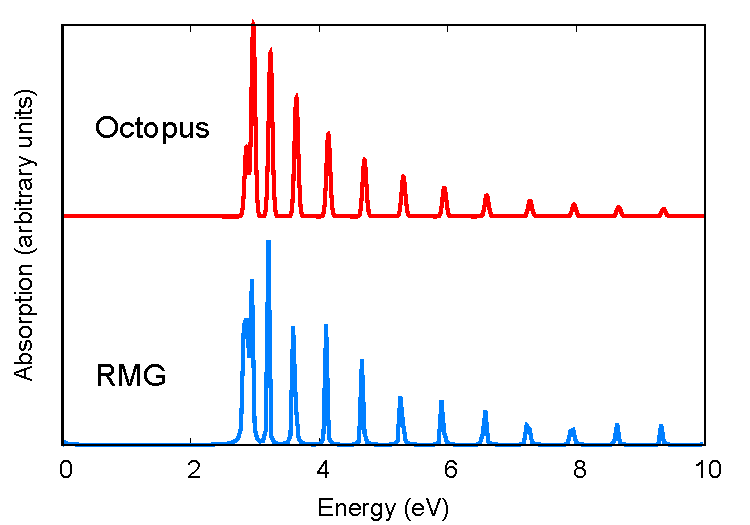
\includegraphics[width=\columnwidth]{Figs/out-h2.pdf}
  \caption{\footnotesize
    \myred{[Caption for H$_2$ chain optical conductivity figure.
    Should describe: (a) longitudinal $\sigma_{zz}(\omega)$ and
    transverse $\sigma_{xx}(\omega)$ components from RMG compared
    with Octopus; (b) convergence with k-point density if shown;
    labels for RMG and Octopus curves.
    Note anisotropy of 1D system as key feature to highlight.]}
  }
  \label{fig:h2}
\end{figure}

\myred{[Discussion points:
- Agreement between RMG and Octopus for both longitudinal and
  transverse components
- K-point convergence: how many k-points needed for converged spectrum?
- Physical interpretation of the spectral features
- If Berry phase comparison is available: show agreement between
  current-integration and BP polarization as internal consistency check
  (Fruit 1 from CONTEXT.md)
- If ground-state current convergence is shown: include as panel or
  note in text (Fruit 2 from CONTEXT.md)]}


%--------------------------------------------------------------------
\subsection{Two-Dimensional Periodic System: Hexagonal Boron Nitride}
\label{sec:hbn}
%--------------------------------------------------------------------

Hexagonal boron nitride (hBN) is a wide-gap insulating two-dimensional
material with $D_{6h}$ symmetry.
Its optical response is highly anisotropic: the in-plane conductivity
$\sigma_{xx}(\omega) = \sigma_{yy}(\omega)$ differs markedly from the
out-of-plane component $\sigma_{zz}(\omega)$, the latter being
negligible for photon energies below the interlayer excitations.
This system tests the implementation of two-dimensional periodic
boundary conditions and the symmetry enforcement of the conductivity
tensor in \texttt{RMG}.

\myred{[Computational details:
- Monolayer geometry: lattice constant \myred{[a]} \AA,
  vacuum layer \myred{[d]} \AA\ to prevent inter-layer interactions
- K-point sampling: \myred{[N\_k $\times$ N\_k $\times$ 1]} Monkhorst-Pack
- Grid spacing: \myred{[value]} a$_0$
- XC functional: \myred{[PBE]}
- Pseudopotential: \myred{[type]}
- Time step and total simulation time: \myred{[values]}]}

\begin{figure}[ht!]
  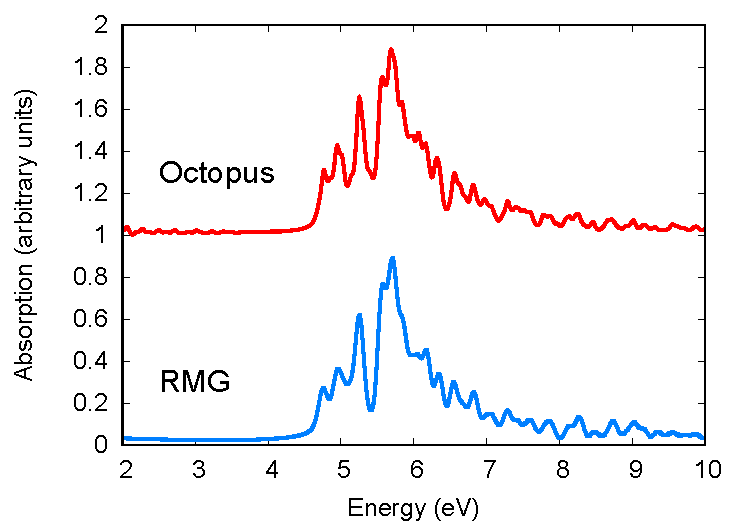
\includegraphics[width=\columnwidth]{Figs/out-hBN.pdf}
  \caption{\footnotesize
    \myred{[Caption for hBN optical conductivity figure.
    Should describe: in-plane $\sigma_{xx}(\omega)$ from RMG and
    Octopus; out-of-plane component if shown; indicate the onset
    of absorption near the band gap.
    Highlight that $\sigma_{xx}=\sigma_{yy}$ (symmetry correctly
    reproduced) and $\sigma_{zz}\approx 0$.]}
  }
  \label{fig:hbn}
\end{figure}

\myred{[Discussion points:
- Agreement between RMG and Octopus for in-plane conductivity
- Symmetry: show that $\sigma_{xx}=\sigma_{yy}$ (Fruit 3 from CONTEXT.md)
- Physical features: onset at band gap, first excitonic peak if visible
- Comparison with available experimental or LR-TDDFT data if relevant]}


%--------------------------------------------------------------------
\subsection{Three-Dimensional Periodic System: Silicon}
\label{sec:si}
%--------------------------------------------------------------------

Silicon in the diamond cubic structure ($F d\bar{3}m$, space group 227)
is the canonical benchmark for periodic electronic structure
calculations.
Its indirect band gap and well-characterized optical spectrum provide
a rigorous test of the full three-dimensional periodic RT-TDDFT
implementation.
The cubic symmetry requires $\sigma_{xx}(\omega) = \sigma_{yy}(\omega)
= \sigma_{zz}(\omega)$, providing an immediate symmetry validation.

\myred{[Computational details:
- Unit cell: conventional 8-atom cell, lattice constant \myred{[a]} \AA
- K-point sampling: \myred{[N\_k $\times$ N\_k $\times$ N\_k]} Monkhorst-Pack
- Grid spacing: \myred{[value]} a$_0$
- XC functional: \myred{[PBE]}
- Pseudopotential: \myred{[type, NCPP]}
- Number of occupied + virtual states: \myred{[N\_occ + N\_virt]}
- Time step $\Delta t$: \myred{[value]} a.u.
- Total simulation time: \myred{[value]} a.u. (\myred{[value]} fs)
- Broadening $\gamma$: \myred{[value]} eV]}

\begin{figure}[ht!]
  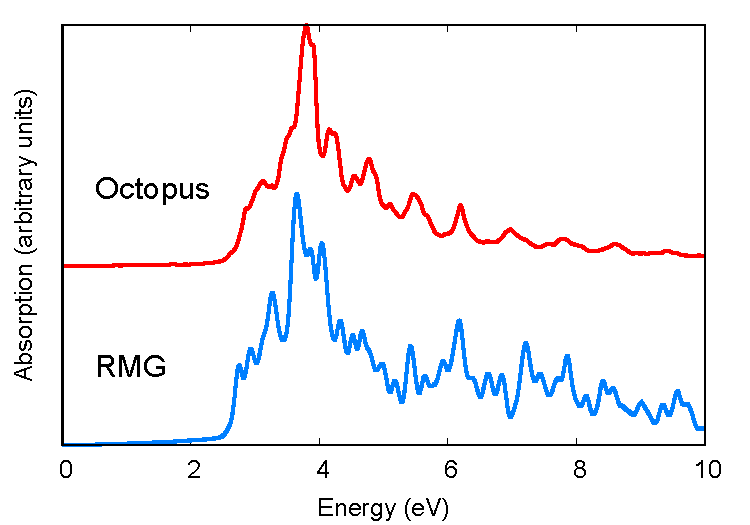
\includegraphics[width=\columnwidth]{Figs/out-Si.pdf}
  \caption{\footnotesize
    \myred{[Caption for Si optical conductivity figure.
    Should describe: $\sigma_{xx}(\omega)$ (= $\sigma_{yy}$ = $\sigma_{zz}$
    by cubic symmetry) from RMG compared with Octopus;
    indicate band gap region; optionally compare with experiment.
    If energy conservation panel included: describe it.]}
  }
  \label{fig:si}
\end{figure}

\myred{[Discussion points:
- Agreement between RMG and Octopus: peak positions, lineshapes
- Symmetry: $\sigma_{xx}=\sigma_{yy}=\sigma_{zz}$ (Fruit 3)
- Energy conservation test for periodic case (Fruit 5 from CONTEXT.md):
  run longer simulation and show no drift, analogous to paper 1 Fig.~3c
- Berry phase comparison if included (Fruit 1)
- Physical features: onset near direct gap, main optical peak structure]}


%--------------------------------------------------------------------
\subsection{Spin-Polarized System: \ch{CrI3}}
\label{sec:cri3}
%--------------------------------------------------------------------

Chromium triiodide (\ch{CrI3}) is a layered van der Waals magnetic
insulator with a honeycomb lattice of \ch{Cr^{3+}} ions, each carrying
a local moment of approximately $3\,\mu_B$.
In its ferromagnetic ground state, the spin-up and spin-down electronic
structures differ, leading to distinct optical spectra for the two
spin channels.
This system provides a direct test of the spin-collinear RT-TDDFT
extension: the two spin channels should propagate independently but
with a common Hartree potential, yielding spin-resolved optical
conductivities that can be compared with \texttt{Octopus} and with
available experimental data.

\myred{[Computational details:
- Unit cell: \myred{[describe geometry and magnetic ordering]}
- K-point sampling: \myred{[N\_k $\times$ N\_k $\times$ N\_k]}
- XC functional: \myred{[PBE or PBE+U; specify U if used]}
- Pseudopotential: \myred{[type, NCPP]}
- Initial spin configuration: ferromagnetic, moments on Cr sites
- Time step and total simulation time: \myred{[values]}
- Broadening: \myred{[value]} eV]}

\begin{figure}[ht!]
  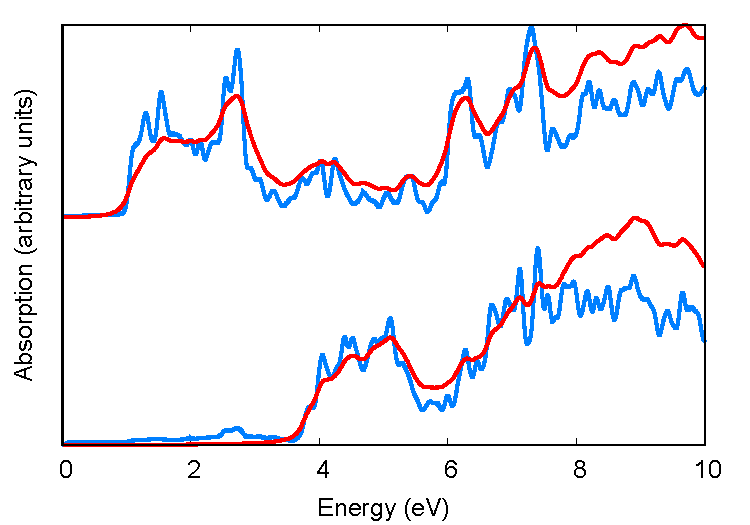
\includegraphics[width=\columnwidth]{Figs/out-CrI3.pdf}
  \caption{\footnotesize
    \myred{[Caption for \ch{CrI3} optical conductivity figure.
    Should describe: spin-up and spin-down optical conductivities
    from RMG compared with Octopus; indicate the relevant spectral
    features (charge-transfer peaks, d-d transitions);
    note that spin channels are labeled consistently.]}
  }
  \label{fig:cri3}
\end{figure}

\myred{[Discussion points:
- Agreement between RMG and Octopus for both spin channels
- Physical interpretation: which spectral features are spin-up vs spin-down?
  Charge-transfer excitations, Cr d-d transitions
- Spin current $\mathbf{J}_{\mathrm{spin}} = \mathbf{J}^\uparrow
  - \mathbf{J}^\downarrow$ if computed (Fruit 4 from CONTEXT.md)
- Comparison with available experimental optical data if relevant
- Note: ECD/MCD spectra not computed in this work (magnetic perturbation
  formalism reserved for future publication)]}


%--------------------------------------------------------------------
\subsection{Large-Scale Demonstration: NV Center in Diamond}
\label{sec:nv}
%--------------------------------------------------------------------

As a demonstration of the unique large-scale capability of \texttt{RMG},
we apply the periodic spin-polarized RT-TDDFT implementation to
nitrogen-vacancy (NV) centers in diamond.
The NV center---a substitutional nitrogen atom adjacent to a carbon
vacancy---is one of the most studied point defects in solid-state
physics, of primary importance for quantum sensing and quantum
information applications due to its long spin coherence time at
room temperature.\cite{nv-center-review}

In a standard periodic DFT or RT-TDDFT calculation, the NV center is
represented by a single defect in a periodically repeated supercell.
The physical properties of the \emph{isolated} defect are recovered
only when the supercell is large enough that the interaction between
the defect and its periodic images is negligible.
Identifying this convergence threshold is both a practical necessity
and a physically meaningful result: it establishes the minimum defect
concentration at which the isolated-defect limit is reached.

We investigate this convergence by performing RT-TDDFT calculations
on diamond supercells containing a single NV center, systematically
increasing the cell size from \myred{[N$_{\min}$] to [\myred{N$_{\max}$}}]
atoms.
\myred{[Specific supercell sizes to be determined. Suggested sequence
(subject to computational feasibility on Frontier):
64, 216, 512, 1000, [larger if possible]
These correspond to defect concentrations of approximately
\myred{[values]} cm$^{-3}$.]}

\myred{[Computational details:
- Host: diamond cubic, lattice constant \myred{[a]} \AA
- Defect: single NV$^-$ center (negatively charged)
- Spin state: triplet ground state ($S=1$), ferromagnetic alignment
- K-point sampling: Gamma point only for large supercells
  (\myred{[note if Gamma+additional k-points used for small cells]})
- XC functional: \myred{[PBE]}
- Pseudopotential: \myred{[NCPP type]}
- Number of states: \myred{[N\_occ + N\_virt per spin]}
- Time step and total simulation time: \myred{[values]}
- Computational platform: Frontier at ORNL
- Nodes used: \myred{[values per system size]}]}

\begin{figure}[ht!]
  \myred{[Figure placeholder: NV center convergence figure.
  Suggested panels:
  (a) Optical conductivity $\sigma(\omega)$ for each supercell size,
      showing convergence with increasing cell size
  (b) Convergence metric vs supercell size (e.g., peak position or
      integrated spectral weight) showing saturation
  (c) Optionally: timing data showing scaling with system size
  Label defect-related spectral features (zero-phonon line region,
  broad phonon sideband).]}
  \caption{\footnotesize
    \myred{[Caption for NV center convergence figure.
    Describe the system, the supercell sizes shown, the key spectral
    features, and the convergence behavior. Identify the minimum
    supercell size for which the isolated-defect optical spectrum is
    recovered within \myred{[tolerance]}.]}
  }
  \label{fig:nv}
\end{figure}

\myred{[Discussion points:
- At what supercell size does the spectrum converge?
  What is the corresponding defect concentration threshold?
- What is the physical origin of the convergence: direct defect-defect
  orbital overlap, or longer-range electrostatic interaction?
- How does the spin-up and spin-down optical response differ?
  Does the convergence behavior differ between spin channels?
- Timing data: how does the computational cost scale with cell size?
  At what size does the TDDFT step dominate over the SCF step?
  (Compare with paper 1 Table 1 format for Ag nanorods.)
- This demonstration establishes the unique position of RMG for
  studying realistic defect concentrations in extended systems.]}
